\documentclass[border=0.8ex,svgnames,varwidth]{standalone}
\usepackage{amsmath,mathtools}
\usepackage{fontspec}
\setmainfont{Source Serif 4}
\setsansfont{Source Sans 3}
\setmonofont{Source Code Pro}
\usepackage{subcaption}
\captionsetup{
  font=scriptsize,
  labelfont=it,
  textfont=rm,
  labelformat=parens,
  position=above,
  labelsep=space,
  justification=centering,
}
\usepackage{tikz}
\usetikzlibrary{positioning}
\begin{document}
\begin{figure}
  \centering
  \begin{subfigure}[b]{0.48\linewidth}
    \centering
    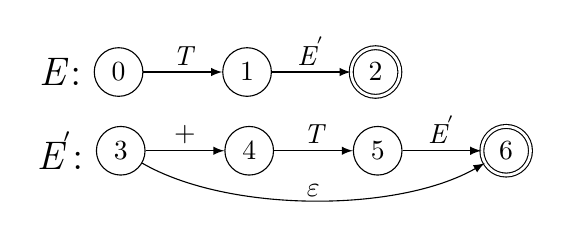
\begin{tikzpicture}
      % E
      \node (E) at (0,0) {\Large \textit{E}:};
      \node[circle,draw=black,right=0.1em of E] (zero) {0};
      \node[circle,draw=black,right=of zero] (one) {1};
      \node[circle,double,double distance=1pt,draw=black,right=of one] (two) {2};

      \path[-latex,draw]
      (zero) edge node[above=-1pt]{\(\textit{T}\)} (one)
      (one) edge node[above=-1pt]{\(\textit{E}^{'}\)} (two);

      % E'
      \node (ESkim) at (0,-1) {\Large \(\textit{E}^{'}\):};
      \node[circle,draw=black,right=0.1em of ESkim] (three) {3};
      \node[circle,draw=black,right=of three] (four) {4};
      \node[circle,draw=black,right=of four] (five) {5};
      \node[circle,double,double distance=1pt,draw=black,right=of five] (six) {6};

      \path[-latex,draw]
      (three) edge node[above=-1pt]{\(+\)} (four)
      (four) edge node[above=-1pt]{\(\textit{T}\)} (five)
      (five) edge node[above=-1pt]{\(\textit{E}^{'}\)} (six);

      \path[-latex,draw]
      (three) edge[out=330,in=210,max distance=3.6em] node[above=-2pt]{\(\varepsilon\)} (six);
    \end{tikzpicture}
    \caption{}
  \end{subfigure}
  \begin{subfigure}[b]{0.48\linewidth}
    \centering
    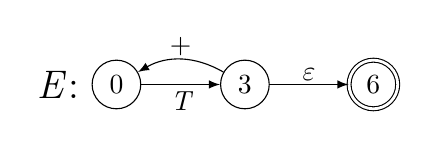
\begin{tikzpicture}
      % E
      \node (E) at (0,0) {\Large \textit{E}:};
      \node[circle,draw=black,right=0.1em of E] (zero) {0};
      \node[circle,draw=black,right=of zero] (three) {3};
      \node[circle,double,double distance=1pt,draw=black,right=of three] (six) {6};

      \path[-latex,draw]
      (zero) edge node[below=-1pt]{\(\textit{T}\)} (three)
      (three) edge node[above=-2pt]{\(\varepsilon\)} (six)
      (three) edge[out=150,in=30,distance=1.2em] node[above=-2pt]{\(+\)} (zero);
    \end{tikzpicture}
    \caption{}
  \end{subfigure}
\end{figure}
\end{document}
